 
\section{Soft-thresholding and Proximal gradient method}
\label{sec:soft-thresholding}
Recall the unconstrained optimization problem
$$
\min _{x} f(x)
$$
We have seen the following results depending on the assumption for $f(x)$
\begin{enumerate}
\item If $f(x)$ is not smooth (for example: $L^1$ norm) which means $\nabla f(x)$ is not continuous, subgradient descent method gives the $\frac{1}{\sqrt{n}}$ convergence.
\item If $f(x)$ is smooth (e.g. $\nabla f(x)$ is L-Lipschitz continuous), gradient descent method gives the $\frac{1}{n}$ convergence. 
\end{enumerate}
There may be other methods (may be for particular functions) which can give better performance. Consider the following example:
$$
f(x)=\frac{1}{2}\|A x-b\|_{2}^{2}+\|x\|_{1}
$$
This is a type 1 problem described above, as the second term is not smooth. However, the objective has a special form. It can be represented as sum of smooth and non -smooth function. Also note that second term $\|x\|_{1}$ is "simple" in a sense that we describe precisely below. In this case, it is conceivable that some tailored method might do better than the generic guarantees offered by sub gradient descent. 

In this section, we introduce what is known as the Proximal method, and show that it provides improved guarantees.  

\subsection{Proximal mapping}\label{sec:proximal}
\begin{definition}
The proximal mapping or prox-operator of a function $f(x)$ is defined as
\begin{equation}\label{pro:def}
\operatorname{Prox}_{f}(x)=\arg \min _{z}f(z)+\frac{1}{2}\|z-x\|_{2}^{2}.
\end{equation}
\end{definition}
Note that $f(x)$ is a convex function so the above problem \eqref{pro:def} a strongly convex problem because of the added Euclidean norm term; therefore the solution is unique. Also for the proximal method to be efficient, we need that $f(x)$ should be simple in the sense that solving the problem \eqref{pro:def}  should be easier and fast or may be even analytical solutions are possible. This condition is required to ensure that each step is not much costly. 

\begin{properties}
From the optimality conditions of minimization in the definition, we can see that $z^*$ is optimal point of $f(x)+\frac12 \|z-x\|_2^2$ only if $0\in \partial f(x) + z^*-x$, namely
\begin{equation}
\begin{aligned}
z^{*}=\operatorname{Prox}_{f}(x) & \Longleftrightarrow 0 \in \partial f(x)+\left(z^{*}-x\right) \\
& \Longleftrightarrow x-z^{*} \in \partial f(x) \\
& \Longleftrightarrow f(w)=f(z)+(x-z)^{T}(w-z)\quad \forall w
\end{aligned}
\end{equation}
\end{properties}
This property shows the relation between proximal mapping  and subgradient of  a function.


\begin{example}
If $f(x)=0$, 
$$
\operatorname{Prox}_{f}(x)=x.
$$
\end{example}
\begin{example}
If $f(x)=|x|$
$$
\begin{array}{l} 
\operatorname{Prox}_{f}(x)=\left\{\begin{array}{cl}
x-1 & \text { if } x\geqslant 1 \\
0 & \text { if } -1 \leqslant x \leqslant 1    \\
x+1 & \text { if } x \leqslant-1
\end{array}\right.
\end{array}
$$	
	\end{example}
\begin{example}
If 
	$$
	f(x)=\left\{\begin{array}{l}
	0 \text { if } x \in[-1,1] \\
	\infty \text { otherwise }
	\end{array}\right.
	$$
$$ 	\begin{array}{l}
	\operatorname{Prox}_{f}(x)=\left\{\begin{array}{cl}
			x & \text { if } x \in [-1, 1] \\
			1 & \text { if } x>1   \\
			-1 & \text { if } x < -1
		\end{array}\right.
	\end{array}  $$
which is the projection onto the set [-1,1].
if $$
f(x)=\left\{\begin{array}{ll}
0 & \text { if } x \in C \\
\infty & x \notin C
\end{array}\right.
$$  these $ \operatorname{prox}_{f}(x) $ is the projection onto C.
	\end{example}
	
%\begin{example}
%	If $ X=\partial f $ where f is convex, what is $ prox_{f} $? 
%	
%	For $ x \subset\mathbb{R}^{d} $, solve for $ (x^{\prime}, y^{\prime}) \in \partial f $ s.t. 
%	$$
%	 x^{\prime}+y^{\prime}=x.
%	$$ Notice that 
%	$$
%	x \in \operatorname{argmin} f \Leftrightarrow 0 \in \partial f(x)
%	$$
%	Also, for $ x \in dom(f_{1}) \cap dom(f_{2}) $, 
%	$$
%	 \partial (f_{1}+f_{2}) (x)=\partial f_{1}(x)+\partial f_{2}(x)  :=\left\{y_{1}+y_{2} ; y_{1} \in \partial f_{1}(x), y_{2} \in \partial f_{2}(x)\right\}
%	 $$ 
%	$$
%	0\in \partial \left(f(z)+\frac{1}{2} \|(x-z)\|^{2}\right)=\partial f(z)-x+z\Rightarrow x \in z+ \partial f(z).
%	$$
%	$$
%	\operatorname{prox}_{f}(x)=\operatorname{argmin}\limits_{z}\left(f(z)+\frac{1}{2}\|x-z\|_2^{2}\right)
%	$$
%	\end{example}
	
\begin{theorem}[soft-thresholding]
Let $f(x)=\lambda\|x\|_1$. Soft-thresholding  is defined as 
\begin{equation}
prox_f(x) = \arg\min_z\{\frac{1}{2}\|x-z\|^2_2 + \lambda\|z\|_1 \},
\end{equation}
which is shown in the following figure
\begin{figure}
\centering
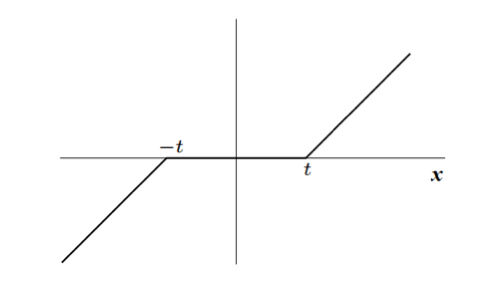
\includegraphics[width=3in]{./6DL/figures/softthreshold}   
%\caption{Two linearly separable sets}
\end{figure}
The $l_1$-norm is is separable in indices. Each $i^{\text {th }}$ coordinate can be optimized separately and the $i^{t h}$ coordinate is given as
$$
prox_f(x)_{i}=\operatorname{sgn}\left(x_{i}\right)\left[\left|x_{i}\right|-\min \left\{\left|x_{i}\right|, \lambda\right\}\right]
=\begin{cases}
0&|x_i|\le \lambda
\\
x_i-\lambda&x_i>\lambda
\\
x_i+\lambda&x_i<-\lambda
\end{cases}.
$$ 
\end{theorem}

\begin{proof}
Note that
\begin{equation}
0 \in \nabla(\frac{1}{2}\|x-z\|^2_2) + \partial(\lambda\|z\|_1) \Leftrightarrow 0 \in z-x + \lambda\partial\|z\|_1
\end{equation}
The $l_1$-norm is separable and thus we can consider each of its components separately. Let's examine first the case where $z_i \neq 0$. Then, $\partial \|z_i\|=sign(z_i)$ and the optimum $z_i^*$ is obtained as
\begin{equation}
0 = z_i-x_i + \lambda sign(z_i) \Leftrightarrow z_i^* = x_i - \lambda sign(z_i^*)
\end{equation}
Note also that if $z_i^* < 0$, then $x_i < -\lambda$ and equivalently if $z_i^* > 0 \Rightarrow x_i > \lambda$. Thus, $|x_i| > \lambda$ and $sign(z_i^*) = sign(x_i)$. Substituting in the previous equation we get 
\begin{equation}
z_i^* = x_i - \lambda sign(x_i)
\end{equation}
In the case where $z_i = 0$, the subdifferential of the $l_1$-norm is the interval $[-1,1]$ and the optimality condition is
\begin{equation}
0 \in -x_i + \lambda[-1,1] \Leftrightarrow x_i \in [-\lambda,\lambda] \Leftrightarrow |x_i| \leq \lambda
\end{equation}
Putting all together we get
\begin{equation}
[prox_f(x)]_i = z_i^* = 
\left\{ \begin{array}{lr} 0 & \text{if } |x_i| \leq \lambda \\ 
x_i - \lambda sign(x_i) &\text{if } |x_i| > \lambda \end{array}\right.
\end{equation}
The previous equation can also be written as
\begin{align*}
[prox_f(x)]_i &= sign(x_i)\max(|x_i|-\lambda, 0) \\
               &= sign(x_i)(|x_i|-\lambda)_+
\end{align*}
where $(\cdot)_+$ denotes the positive part and it leads to sparse solution.
\end{proof}

\subsection{Properties of the proximal map}	
\begin{definition}
: A map g:$ \mathbb{R}^{d} \rightarrow \mathbb{R}^{d} $ is called 
\begin{itemize}
	\item Non-expansive if $ \|g(x)-g(y)\| \leqslant\|x-y\| $
	\item Firauly Non-expansive if $ \|g(x)-g(y)\|^{2} \leqslant\langle g(x)-g(y), x-y\rangle $
	\item A contraction if $ \|g(x)-g(y)\| \leqslant \lambda\|x-y\| \quad \text { for } 0 \leqslant \lambda<1 $
\end{itemize}
\end{definition}

\begin{lemma}
	If g is non-expansive, the $ \frac{1}{2}(g+I) $ is 	firmly non-expansive.
	$$
	\frac{1}{2}(g+I)(x)=\frac{1}{2}(g(x)+x)
	$$
	If g is firmly non-expansive, then $ 2g-I $ is non-expansive.
\end{lemma}

\begin{proof}
	$$
	\begin{aligned}
	\|h(x)-h(y)\|^{2}&=\left\langle\frac{1}{2}[g(x)+x]-\frac{1}{2}[g(y)+y], \frac{1}{2}[g(x)+x]-\frac{1}{2}[g(J)+y]\right\rangle\\
	&=\left\langle\frac{1}{2}(g(x)-g(y))+\frac{1}{2}(x-y), \frac{1}{2}(g(x)-g(y))+\frac{1}{2}(x-y)\right\rangle \\
	&=\frac{1}{4} \|g(x)-g(y)\|^{2}\|x-y\|^{2}+\frac{1}{2}(g(x)-g(y), x-y)+\frac{1}{4}\|x-y\|^{2} \\
	& \leqslant \frac{1}{2}\|x-y\|^{2}+\frac{1}{2}\langle g(x)-g(y), x-y\rangle \\
	&=\left\langle\frac{1}{2}(g(x)-g(y))+\frac{1}{2}(x-y), x-y\right\rangle\\
	&=\langle h(x)-h(y), x-y\rangle .
	\end{aligned}
	$$	
	\end{proof}

\begin{example}
	Non-expansive $ \mathbb{R}^{2}  $, rotate by $ \theta $, has a fixed point, but we don't converge to it.
	Nonexpansive maps may fail to converge to fixed points. Firmly nonexpanisve maps always converge to their fixed points.
	Fixed points may not be unique though.
	\end{example}

\begin{example}
	$ g: \mathbb{R} \rightarrow \mathbb{R}$, 
	$$  g(x)=\left\{\begin{array}{cl}
	x & \text { if } x\in [-1,1] \\
	1 & \text { if }  x > 1    \\
	-1 & \text { if } x <-1
	\end{array}\right.$$
	\end{example}
g is firmly non-expansive. Set of fixed points [-1,1]
\begin{theorem}
The proximal map is always firmly non-expansive.	
	\end{theorem}
\begin{theorem}
If g is firmly nonexpansive and $ g(y)=y $	for some y, there if $ x_{n+1}=g(x_{n}) $,we have $ x_{n} \rightarrow y^{\prime} $ with $ g(y^{\prime})=y^{\prime} $
\end{theorem}

\begin{example}
$ g: \mathbb{R} \rightarrow \mathbb{R}, g(x)=x+1$ is firmly non-expansive in fact $ g(x)=prox_{f}(x), f(x)=-x$
	\end{example}
	
\subsection{Proximal gradient method}	
Proximal point algorithm: 
$$ 
x_{n+1}=prox_{f}(x_{n}).
$$ 
By the preceding if $ prox_{f}$ has a fixed point, then $ x_{n} $ converge to a fixed point.
A fixed point of $ prox_{f}$ is a point x with $0 \in \partial f(x) $, which is a minimizer.
Usually calculating $ prox_{f}$ is just as difficult as minimizing $f$ itself,
$$
prox_{f}=\mathop{argmin}\limits_{z} \frac{1}{2}\|x-z\|_2^{2}+f(z)
$$
%Later we will use 	$ prox_{f}$ and $ prox_{g}$ to construct a firmly non-expansive map whose fixed points mininize $g+h $ Douglas-Rachfound splitting.
%$$
%x_{n+1}=x_{n}-s h_{n}, \quad h_{n}=\mathop{argmax}\limits_{\|h\|_{1}}\left\langle h,\nabla f\left(x_{n}\right)\right\rangle
%$$
%Boosting: $$ \mathop{argmax}\limits_{h \in D}\left\langle h,\nabla f\left(x_{n}\right)\right\rangle $$ 
%If $
%f(x)=\frac{1}{2}\left\|x-x_{0}\right\|^{2}
%$get greedy approx.


Consider unconstrained problem with cost function split in two components
$$
\min f(x)=g(x)+h(x)
$$
where $h$ is convex and differentiable, 
$g$ is convex and possibly nondifferentiable, with inexpensive pro-operator.
The proximal gradient algorithm is
$$
x^{(k)}=\operatorname{prox}_{t_{k} g}\left(x^{(k-1)}-t_{k} \nabla h\left(x^{(k-1)}\right)\right)
$$
where $t_{k}>0$ is step size, constant or determined by line search. Note that if $g(x)=0$, then this method reduces to a gradient descent method.

If we apply the proximal mapping to update rule,
$$
\begin{aligned}
x^{+} &=\underset{z}{\operatorname{argmin}}\left(g(z)+\frac{1}{2 t}\|z-x+t \nabla h(x)\|_{2}^{2}\right) \\
&=\underset{z}{\operatorname{argmin}}\left(g(z)+h(x)+\nabla h(x)^{T}(z-x)+\frac{1}{2 t}\|z-x\|_{2}^{2}\right).
\end{aligned}
$$
This means that
$x^{+}$ minimizes $g(z)$ plus a simple quadratic local model of $h(z)$ around $x$.

\begin{properties}
If 
$$
u=\operatorname{prox}_{f}(x), v= \operatorname{prox}_{f}(y),
$$
then 
$$
(u-v)^{T}(x-y) \geq\|u-v\|_{2}^{2}.
$$
This implies that 
$$
x-u \in \partial f(u), \quad y-v \in \partial f(v) \quad \Longrightarrow \quad(x-u-y+v)^{T}(u-v) \geq 0,
$$
and 
$$
\left\|\operatorname{prox}_{f}(x)-\operatorname{prox}_{f}(y)\right\|_{2} \leq\|x-y\|_{2}
$$
$prox_{f}$ is nonexpansive or Lipschitz continuous with constant 1.
\end{properties}

\begin{definition}
	 The proximal map of X, $ prox_{X}(x)=x^{1} $(" Backward Euler")
\end{definition}




%\begin{remark}
%\begin{enumerate}
%\item If the full gradient descent method is used, $\eta$ is a given value.
%\item If the stochastic  gradient descent method is used, $\eta$ is approaching 0 as t goes to infinity. We don't expect sparse 'minimization sequence'
%\item Can we find a different training algorithm that would give 'sparsity'?
%\end{enumerate}
%\end{remark}


%\section{Forward-Backward Splitting Algorithm(not included)}
%\begin{lemma}
%$\Theta=\{\theta:f(\theta,x)\ \text{ is a classifier}\}$ is a non-empty open set.
%\end{lemma}
%
%
%\begin{remark}
%\begin{enumerate}
%\item Question 1: Can we find some sparse $\theta\in \Theta$ by certain training algorithm?
%\begin{itemize}
%\item The desirable training algorithm should converge.
%\item The desirable training algorithm generates 'sparse' minimization sequence.
%\end{itemize}
%
%\item Question 2: Can we find a model $L(\theta)+R(\theta)$ with small $R(\theta)$ s.t. $\arg\min(L(\theta)+R(\theta)) \approx \arg\min L(\theta)$.
%\end{enumerate}
%\end{remark}
%A general approach is to use $L(\theta)+R(\theta)$, where $R(\theta)=\lambda \|\theta\|_1$.
%
%Assume f is strongly convex and smooth function and R is convex. Thus $x^*= \arg\min (f(x)+R(x)) \iff 0\in \nabla f(x^*)+\partial R(x^*)$.
%We have the following forward-backward splitting algorithm.

%\section{A summary of algorithms and convergence results}
%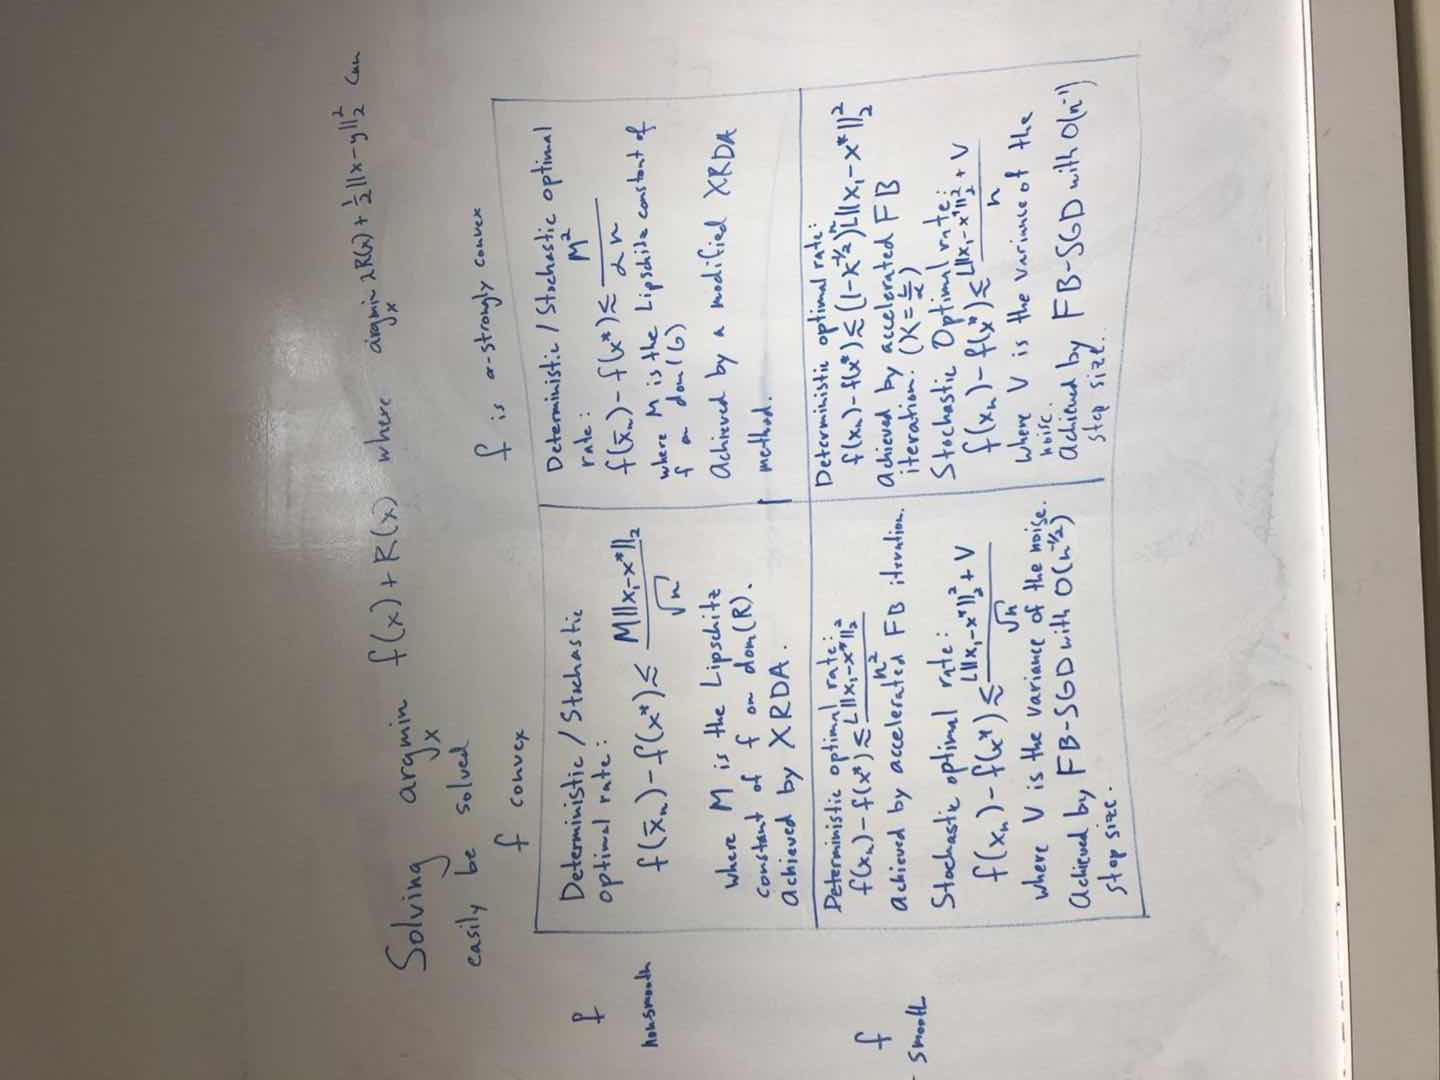
\includepdf[pages=-,angle=270]{6DL/SGD-summary.jpeg}

